\documentclass[letterpaper,12pt]{article}

\usepackage[top=1in, left=1.25in, right=1.25in, bottom=1in]{geometry}
\usepackage[utf8]{inputenc}
\usepackage[T1]{fontenc}
\usepackage[spanish]{babel}
\usepackage{graphicx}
\usepackage{float}

\usepackage{biblatex}

\begin{document}

\tableofcontents
\clearpage

\section{Introducción}

\begin{itemize}
\item \textbf{Planteamiento del Problema:} Crear un documento básico conjunto en LaTeX y un repositorio compartido en GitHub.
\item \textbf{Motivación:} La importancia de resolver este problema radica en poder dominar la creación de documentos en Overleaf para conseguir así un formato mucho más limpio y organizado en los reportes. Así mismo, es necesario aprender a usar GitHub para tener un control de versiones de un documento creado en Overleaf.
\item \textbf{Objetivos:} Aprender las funciones básicas de LaTex y GitHub para el desarrollo de documentos colaborativos.
\end{itemize}
\section{Marco Teórico}
LaTeX: Es un sistema de gestión y desarrollo de textos basada líneas de código y reglas de sintaxis básicas para la edición de un documento.

GitHub: Es una herramienta que lleva el control de las versiones de un archivo (qué se modificó y quién lo hizo), permite la colaboración en equipo para crear proyectos.

\section{Desarrollo}
Para iniciar el desarrollo de la práctica, hicimos un repositorio de GitHub y nos agregamos como colaboradores para que todos podamos ver y editar el repositorio. Creamos las cuentas de Overleaf que usaremos para hacer las prácticas de LaTeX y comenzamos a hacer el documento con la invitación de la cuenta que tiene Overleaf premium.
Posteriormente fuimos trabajando en la práctica siguiendo los lineamiento de entrega de reportes, atendiendo cuidadosamente las reglas de sintaxis y comandos de Overleaf.

Finalmente sincronizamos una de las cuentas a Github y mediante los comandos de Git, subimos el código de nuestro documento al repositorio

\section{Resultados}

\begin{figure}[H]
    \centering
    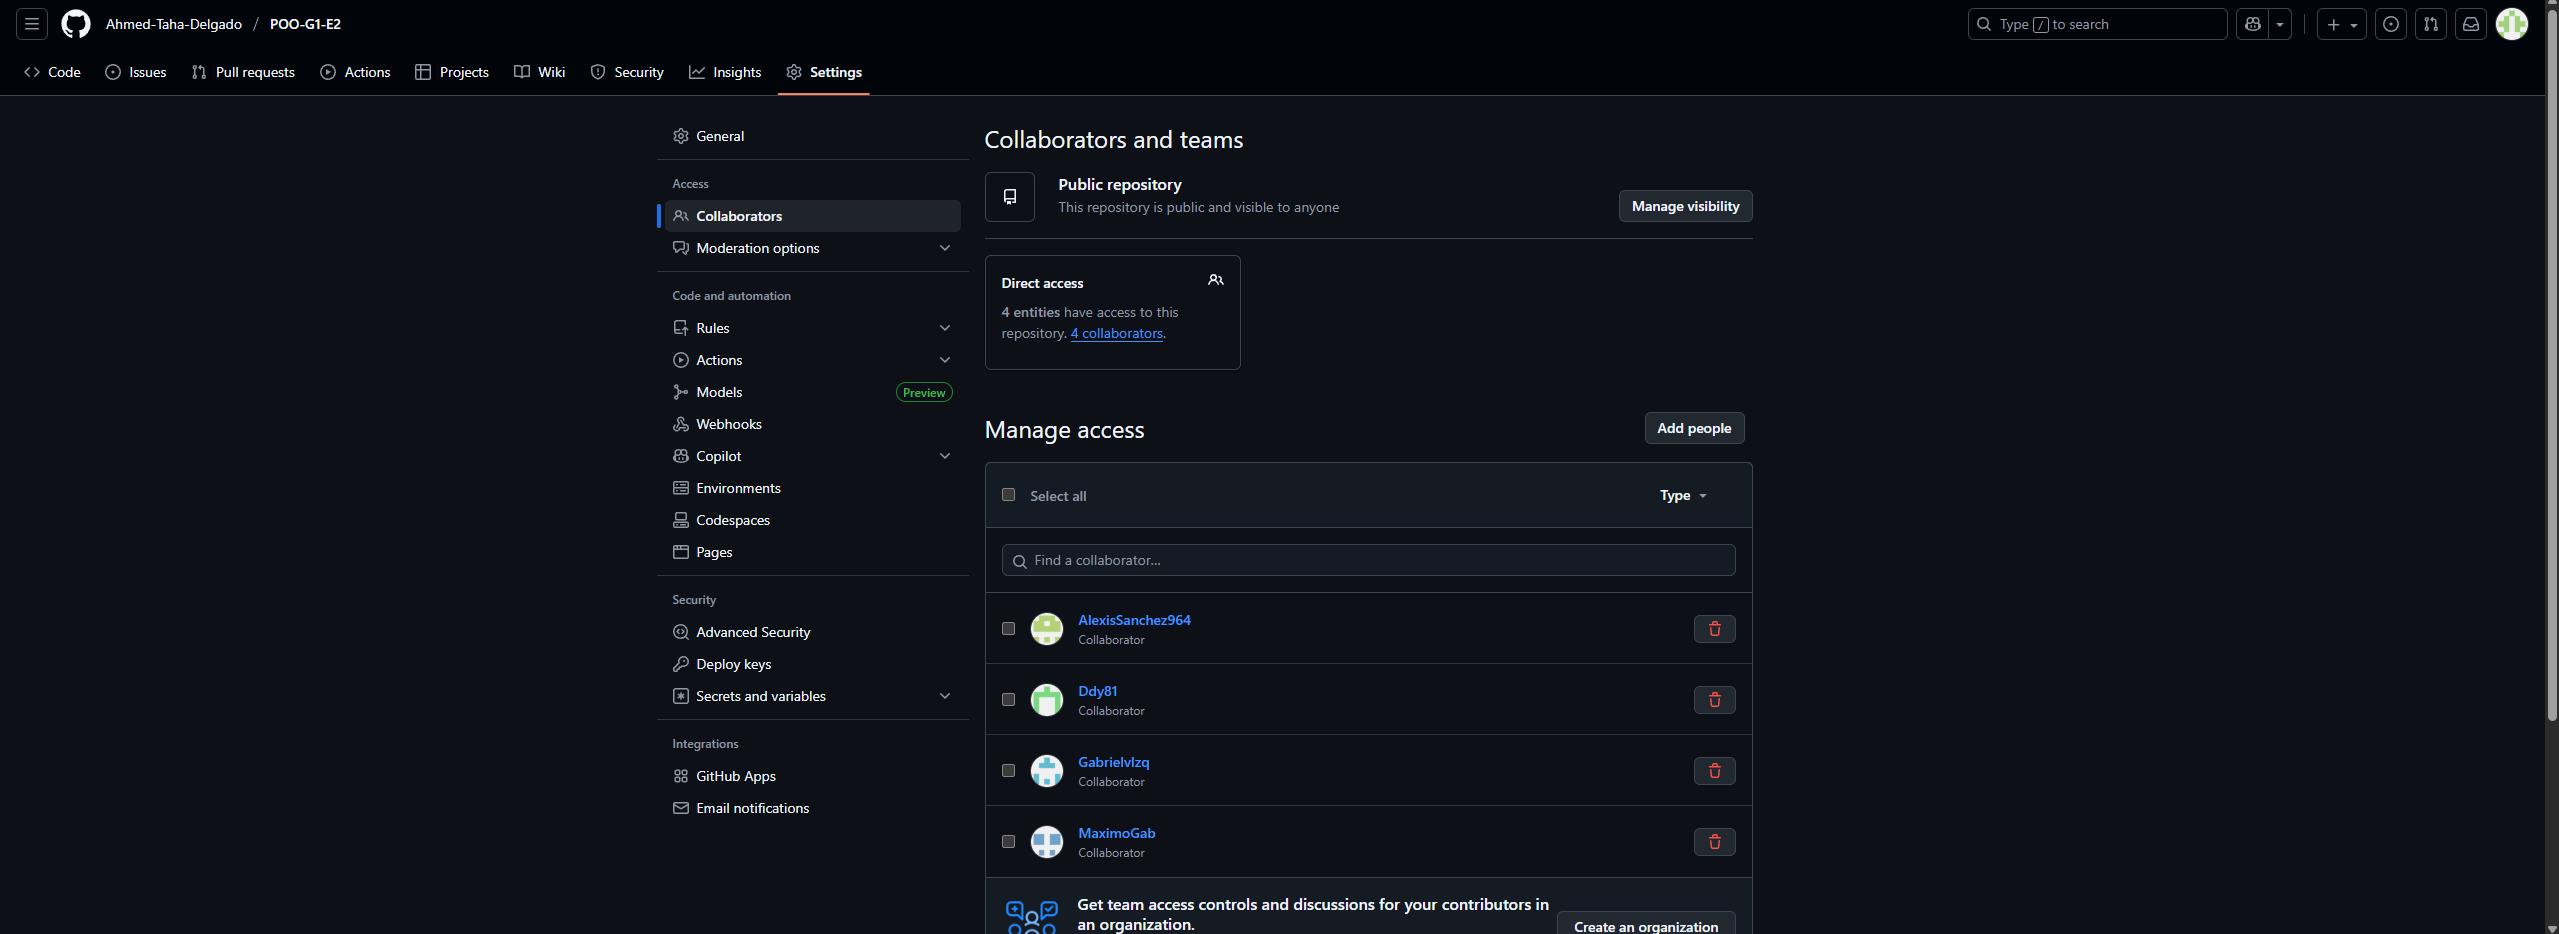
\includegraphics[width=14cm]{Colaboradores.png}
    \caption{Captura de pantalla del repositorio de GitHub con los colaboradores}
    \label{fig:colaboradores}
\end{figure}


\begin{figure}[H]
    \centering
    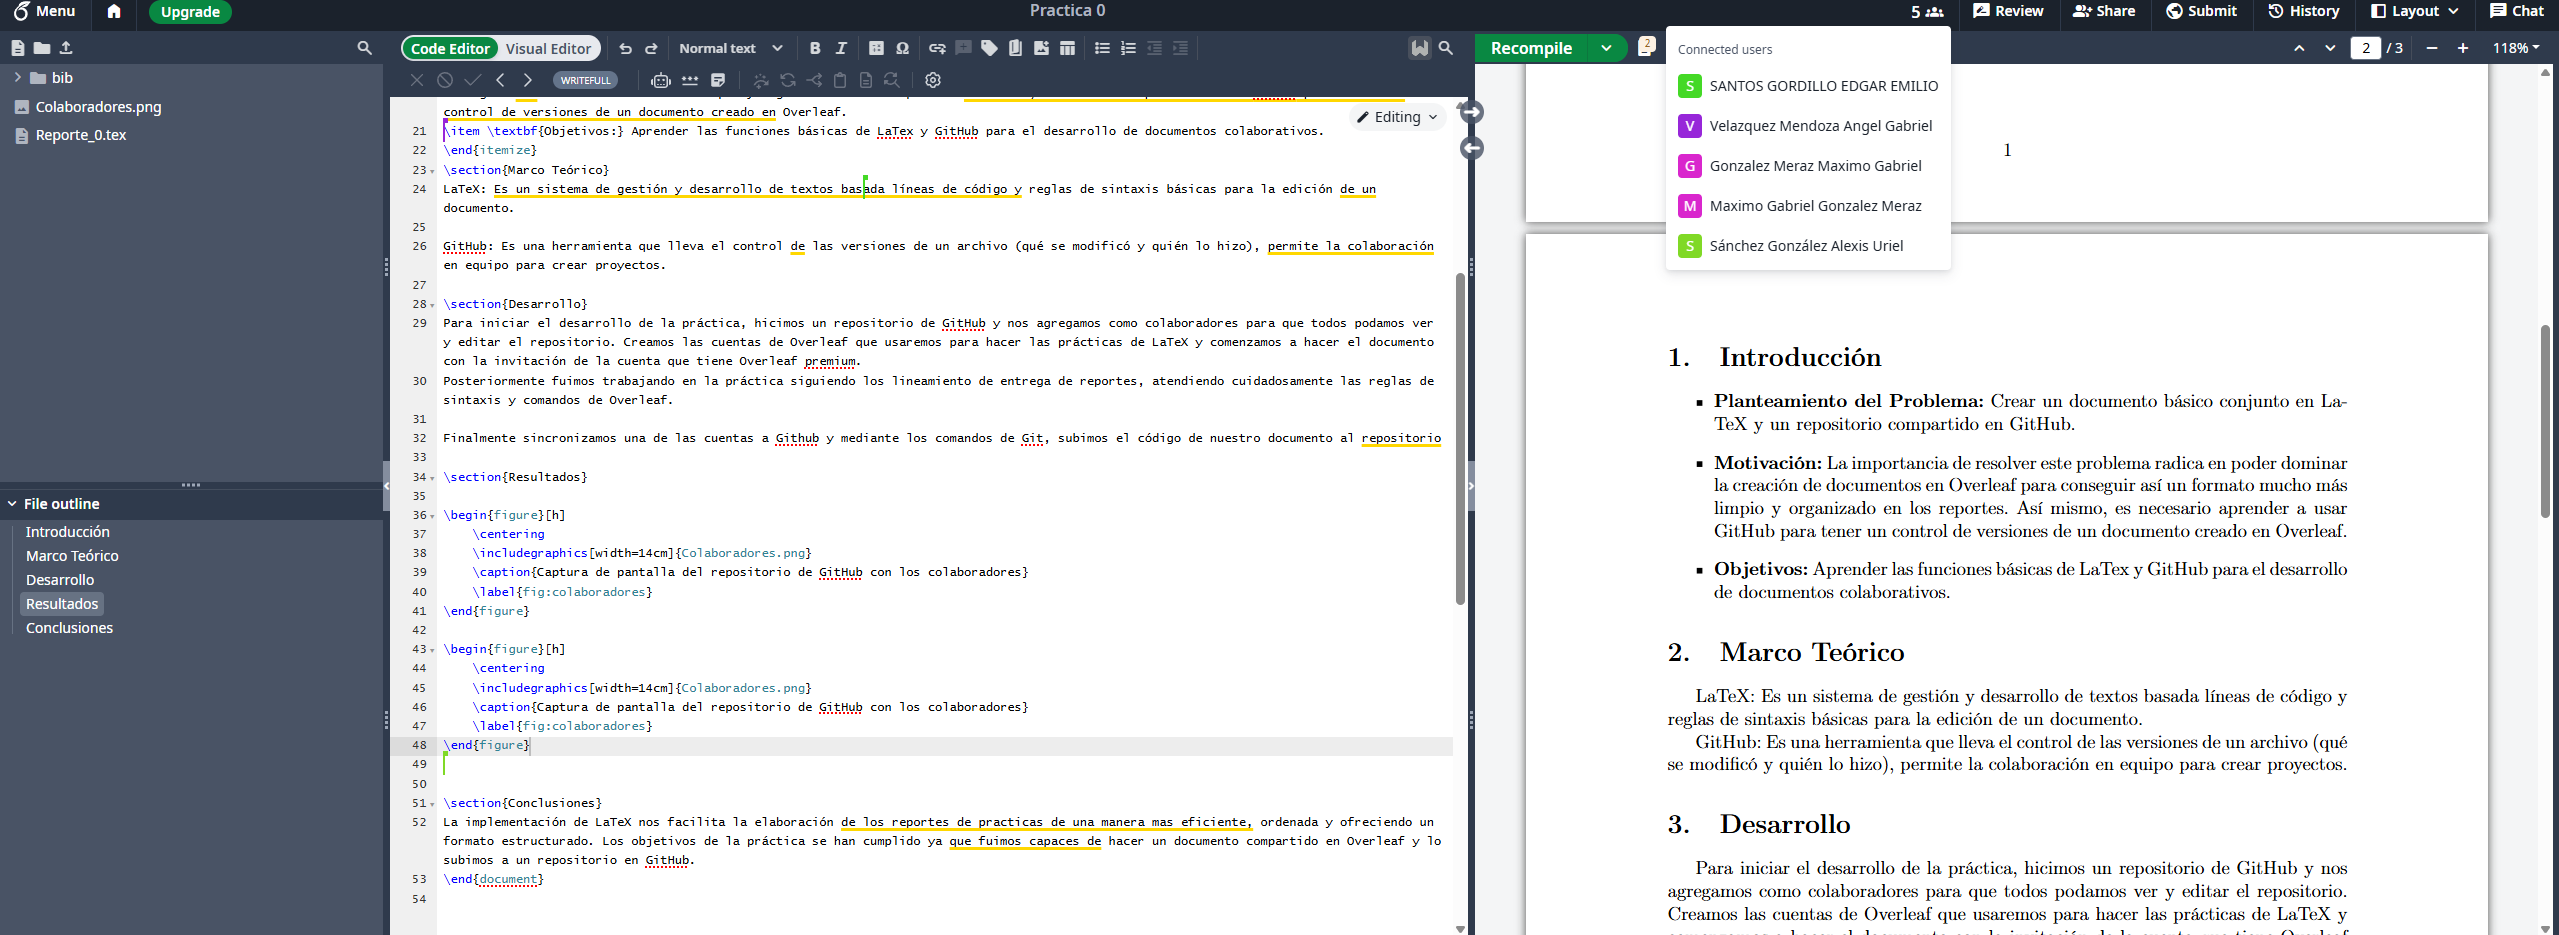
\includegraphics[width=14cm]{Edicion.png}
    \caption{Captura de pantalla del equipo trabajando en el documento}
    \label{fig:colaboradores}
\end{figure}

A continuación están las capturas de como subimos el código de overleaf desde comandos de git al repositorio:

\section{Conclusiones}
La implementación de LaTeX nos facilita la elaboración de los reportes de practicas de una manera mas eficiente, ordenada y ofreciendo un formato estructurado. Los objetivos de la práctica se han cumplido ya que fuimos capaces de hacer un documento compartido en Overleaf y lo subimos a un repositorio en GitHub.

\section{Reto para token}


\begin{center}
    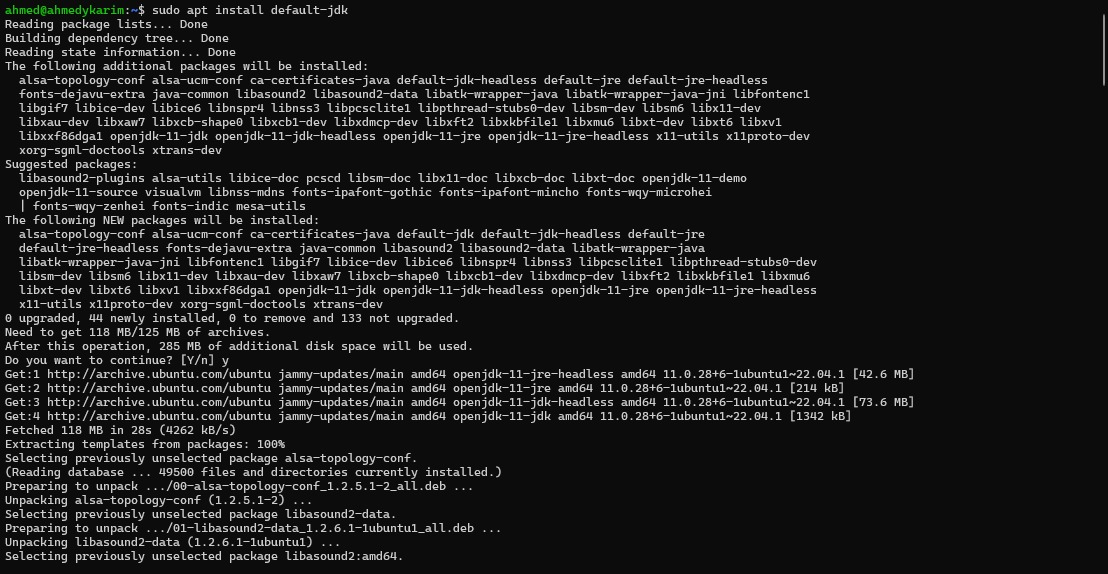
\includegraphics[width=14cm]{descarga1.jpeg}
\end{center}

\begin{figure}[H]
    \centering
    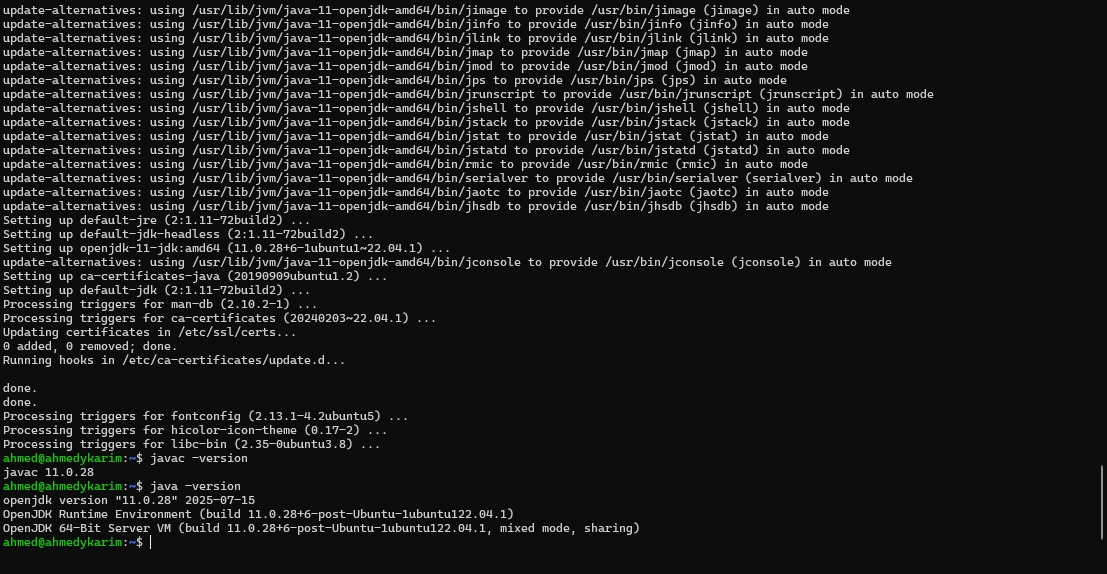
\includegraphics[width=14cm]{descarga2.jpg}
    \caption{Descarga de Java en WSL}
    \label{fig:java}
\end{figure}

\begin{figure}[H]
    \centering
    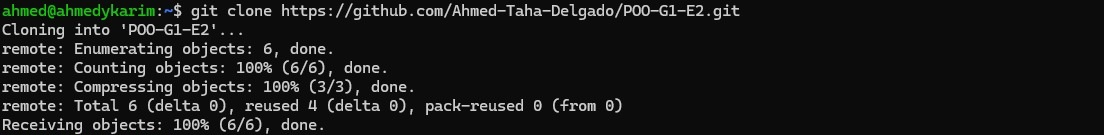
\includegraphics[width=14cm]{clonar.jpeg}
    \caption{Clonación del repositorio de GitHub}
    \label{fig:java}
\end{figure}

\begin{figure}[H]
    \centering
    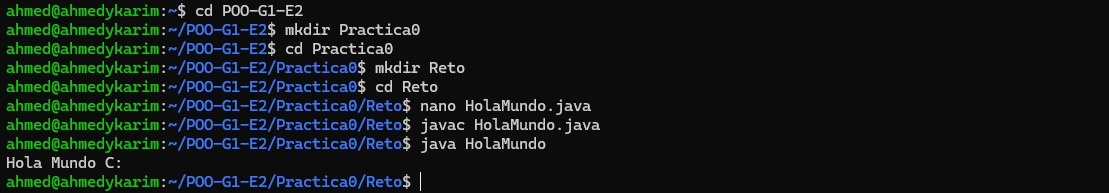
\includegraphics[width=14cm]{creacion.jpeg}
    \caption{Creación de los directorios y archivos y ejecución del Hola Mundo en java}
    \label{fig:java}
\end{figure}

\begin{figure}[H]
    \centering
    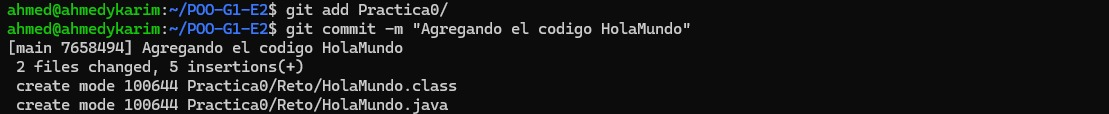
\includegraphics[width=14cm]{commit.jpeg}
    \caption{Commit del repositorio a Git}
    \label{fig:java}
\end{figure}

\begin{figure}[H]
    \centering
    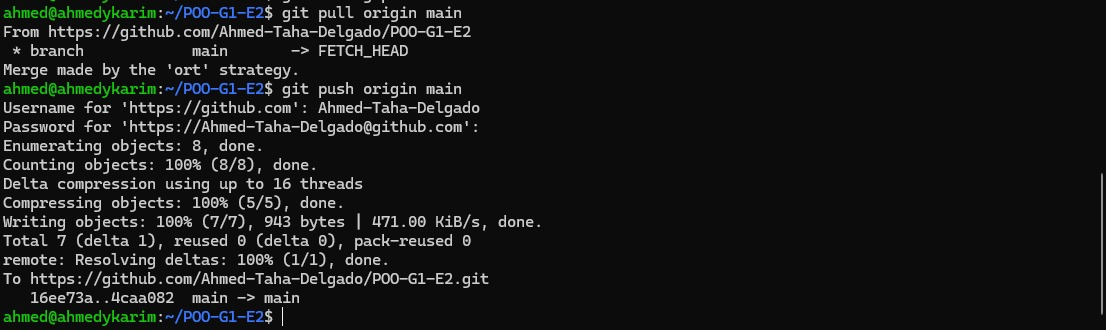
\includegraphics[width=14cm]{push.jpeg}
    \caption{Push del repositorio}
    \label{fig:java}
\end{figure}

\begin{figure}[H]
    \centering
    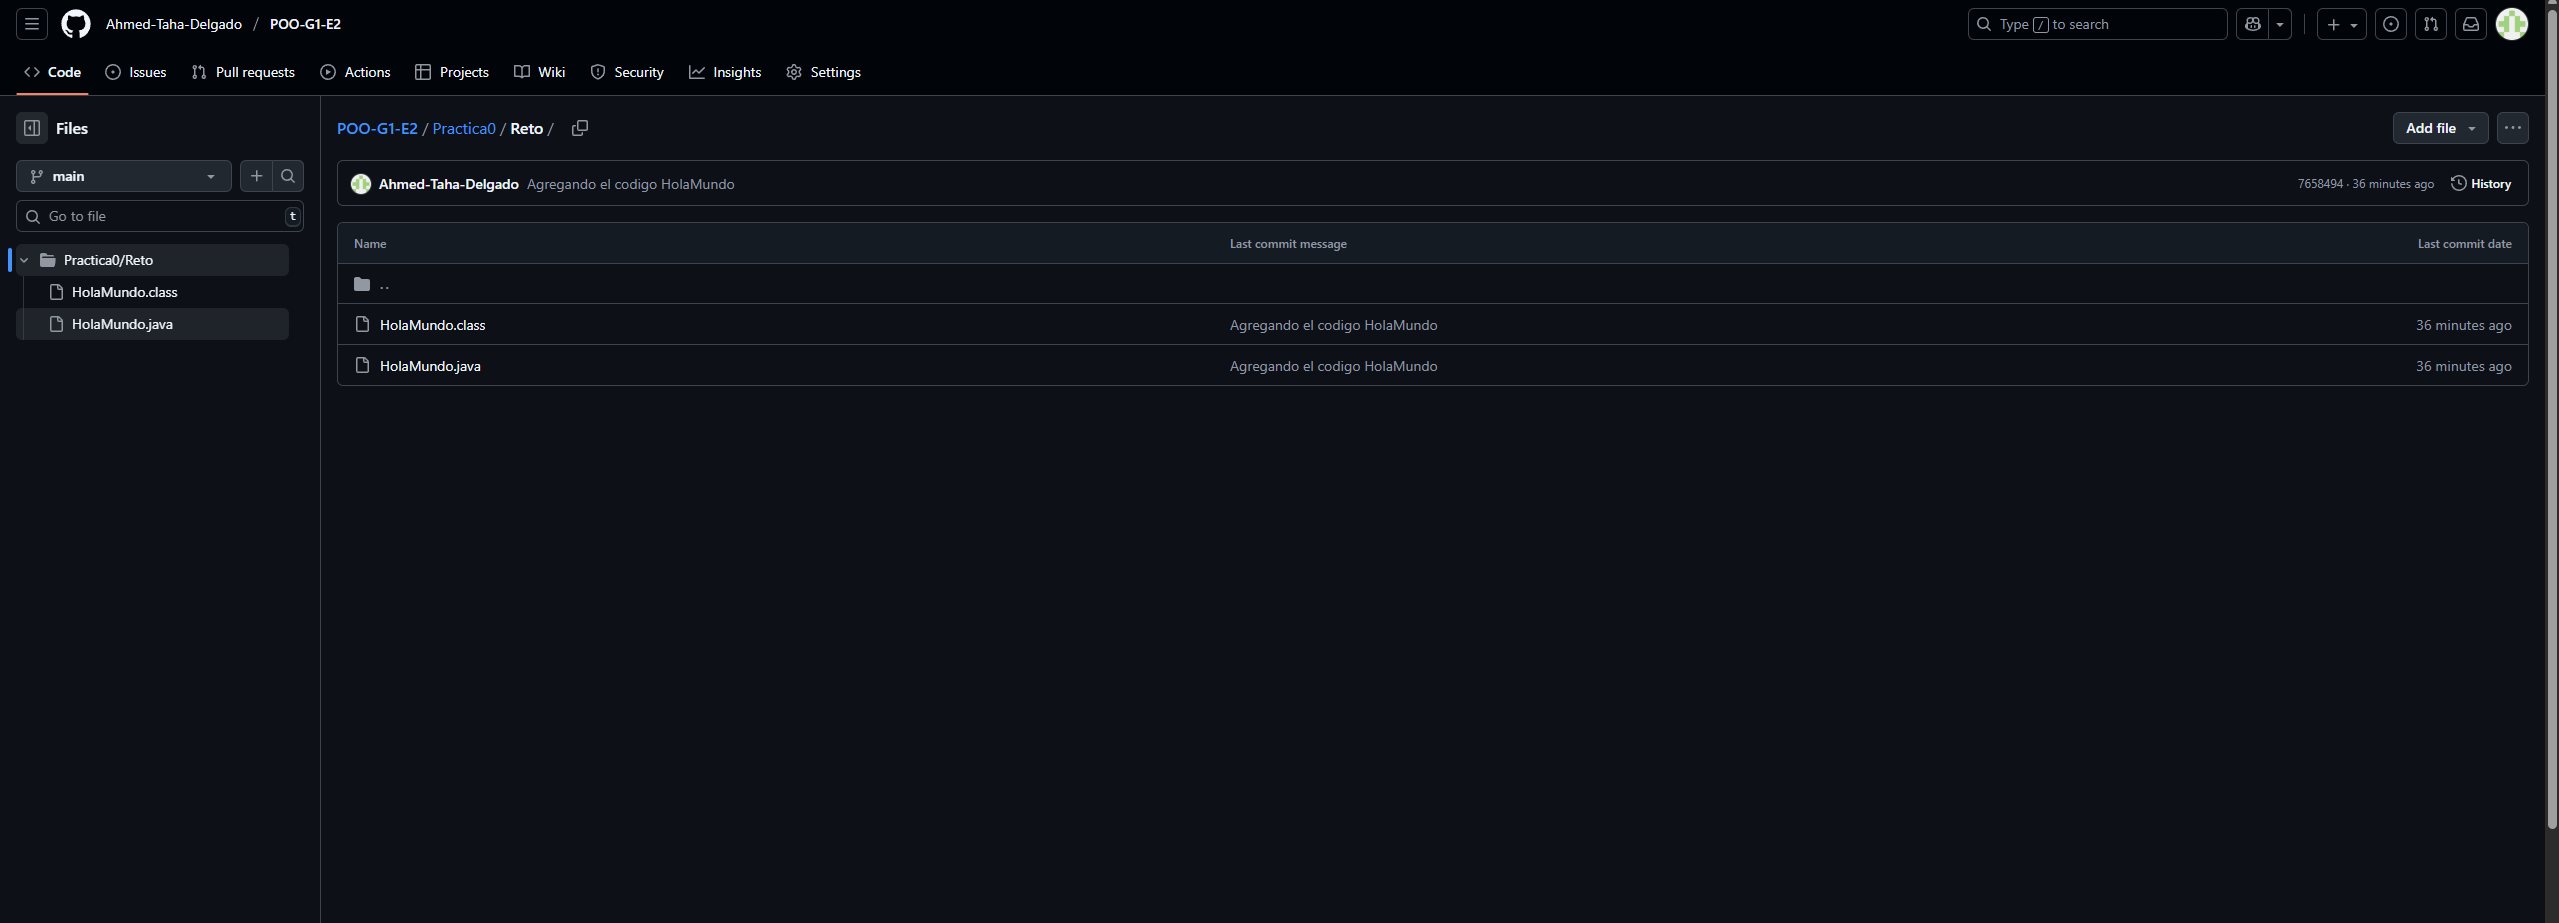
\includegraphics[width=14cm]{repo.png}
    \caption{Repositorio de GitHub actualizado}
    \label{fig:java}
\end{figure}

\end{document}